% ----------------------------------------------------------------
\section{Introduction}
\label{sec:introduction}

\input 01intro

\section{Step 1: The Basics}

\input 02step1

\section{Step 2: Blocking}

\input 03step2

\section{Step 3: GOTO paper: Combine Step1 (small matrice for kernel) and Step2 (blocking for framework)}

\input 04step3

% ----------------------------------------------------------------
\section{The Goto Approach to Implementing {\sc gemm}}
\label{sec:BLIS}

\begin{figure}[tb!]
\begin{center}
\begin{minipage}{3in}
\mbox{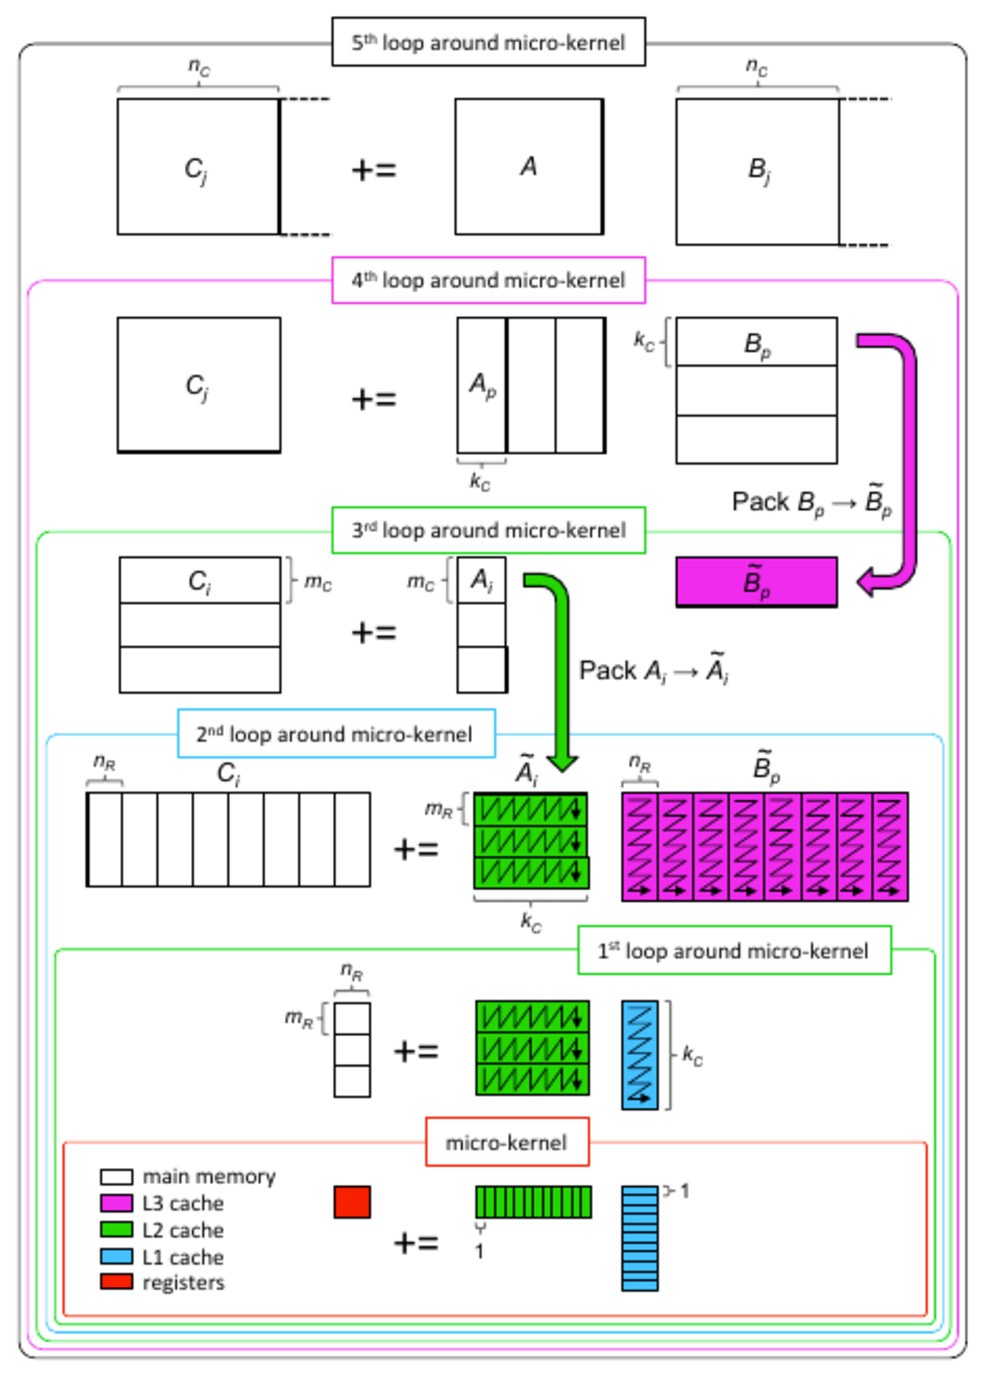
\includegraphics[width=3.0in]{mm_blis_color.pdf}}
\end{minipage}
~~~
\begin{minipage}[t]{3in}
\footnotesize  
\mbox{\input blis_gemm_new  }
\end{minipage}
\end{center}
\caption{Left: The Goto algorithm for matrix-matrix multiplication as  
  refactored in BLIS.  Right: the same algorithm, but expressed as  
  loops.}
\label{fig:blis_gemm}
\end{figure}

\cite{Goto:2008:AHP}
\cite{BLIS1}
\cite{BLIS2}
\cite{BLIS3}
\cite{BLIS4}

\section{Organization of the Project}

\input DirectoryTree

One goal of this exercise is to teach the reader how a software library project is often organized into directories.  We acknowledge that the structure is probably overkill for this relatively simple situation, but hope that it has value nonetheless.



% ----------------------------------------------------------------
% Architecture: Ivy Bridge and Haswell.

\section{Naive Approach: Three loops}



\section{Cache Blocking: 6 loops}

refer to GOTO paper: How to permuate to get the best loop order
var2, var1, var3


Performance Graph

\section{Add packing}


\section{Kernel Tricks}
1. Butterfly or Broadcasting?

2. Double buffering



\section{Parameter Tuning}




\section{Parallelization}










% ----------------------------------------------------------------
\section{Conclusion}
\label{sec:conclusion}

Conclusion.


\subsection*{Additional information}

For additional information on FLAME visit
\begin{center}
\href{http://www.cs.utexas.edu/users/flame/}
     {\tt http://www.cs.utexas.edu/users/flame/}.
\end{center}
